\emph{Draft --- 2026-10-30. Every number in this draft is traceable to a file listed in \path{reports/snapshot.json}.}

\begin{abstract}
Maritime images are rarely degraded by one factor at a time: haze, cloud and sun glare co-occur, yet maritime robustness studies vary one degradation at a time. We introduce a paired evaluation protocol for compound degradations, applied to fine-grained ship-type recognition on FGSC-23 (eight civilian classes): preprocessing is fixed, each image's corruption instance is a deterministic function of its identity, and every condition is evaluated per image, so any two models --- or conditions --- can be differenced without confounding. Four backbone families show compound conditions dropping accuracy by up to 43 points, non-linearly in the single-factor drops. In a pre-registered four-severity design, the compound drop is indistinguishable from its additive prediction at severities 2--4, but at severity 5 it exceeds that prediction by \textbf{+11.3 pp (95\% CI [+7.2, +15.3], BH q < 0.001)} and exceeds the largest single-degradation drop in \textbf{6 of 6} runs. Against the stronger baseline --- the union of the constituents' error sets --- \textbf{41.5\%} of severe-compound errors are made by no single degradation at any severity.

We then ask what removes the excess. Training on calibrated compound samples from six families reduces the excess on three pairs held out of every pool from \textbf{+8.2 pp to $-$1.8 pp} (clean accuracy 84.95\% $\to$ 86.25\%); a control showing the model the same six families one at a time, at the same rate and budget, stays at +7.2 pp (paired-minus-singles \textbf{$-$5.8 pp, 6 of 6 cells}). An arm matched on per-image damage recovers about 60\% of the gain, so the accounting is roughly 60\% under-matched damage and 40\% co-occurrence; the co-occurrence part survives matching (\textbf{$-$3.7 pp, 6 of 6}) and is what transfers to unseen pairs. Neither part transfers to families absent from all pools, as pre-registered. Eight single-point interventions (seven mechanisms plus an initialization control) do not beat a strong combined-augmentation baseline, and we document one artefact that matters beyond this task: a +1.66 pp gain at a 24-epoch screening budget becomes $-$0.18 pp at 40 epochs. We release the protocol, harness, checkpoints and a manifest that reproduces every number.

\textbf{Keywords:} maritime computer vision; ship classification; robustness evaluation; compound degradations; superadditivity; negative results

\end{abstract}

\section{Introduction}
A ship photographed from shore in the Yellow Sea is not degraded by either haze or glare; it is degraded by some mixture of both, on top of an unknown amount of cloud. Recognition models deployed on such imagery are therefore evaluated under conditions that no single-corruption benchmark represents.

The published maritime literature has moved in the opposite direction. FoggySea isolates sea fog \cite{yang2026foggysea}, CARP isolates cloud occlusion \cite{zhan2025carp}, and studies of haze on warship classification isolate haze. Benchmarks that do consider multiple corruptions --- ImageNet-C \cite{hendrycks2019imagenetc} and its descendants --- hold the number of \emph{types} at one and vary only severity. Recent general-vision work studies composition as "two or more corruptions applied in sequence", without decomposing the joint effect against the marginals of its parts. As far as we can establish, no maritime study reports how a compound degradation compares to its constituents, and no study in any domain reports an explicit factorial decomposition of accuracy loss on ship-type recognition.

We therefore ask a narrower question than "how robust are ship classifiers": \textbf{what does a compound degradation do that its constituents do not, and how does that difference depend on severity?}

Answering it required three design decisions that turned out to matter more than any model:

\begin{enumerate}
\item \textbf{Paired corruption.} The corruption parameters for an image are drawn from \texttt{stable\_seed(recipe\_version, sample\_id, role, kind, severity, domain)}. Two models evaluated on the same condition see the identical corrupted image; two conditions evaluated on the same model differ only in the degradation. This turns every model comparison into a paired comparison and removes most of the seed noise that otherwise dominates at 157 validation images.
\item \textbf{Pre-registered screening with full-budget confirmation.} Screening statistics were fixed before training. The protocol's value is shown by the fact that it caught its own artefact: a candidate that looked like +1.66 pp at a 24-epoch budget was $-$0.18 pp at 40 epochs.
\item \textbf{Analysis of stored predictions, not just aggregates.} Every condition's per-image prediction is archived, which lets us ask questions that aggregate accuracies cannot answer --- in particular whether compound failures are the same failures a single degradation makes.
\end{enumerate}
\textbf{Contributions.}

\begin{itemize}
\item A paired protocol for compound-degradation evaluation in maritime recognition, with a strong combined-augmentation baseline, group-disjoint folds and cluster bootstrap inference (§3).
\item Evidence that the effect of compound degradation is \textbf{not} separable into its constituents, and that under the shipped renderer this non-separability appears as a \textbf{threshold confined to the highest severity} rather than a smooth gradient (§4.3) --- including one pre-registered prediction that failed. A physically-motivated renderer, applied to a frozen model and to models retrained under it, reproduces the severity-5 excess (10.2 / 16.0 pp against 9.7 / 12.6 pp) but produces it from severity 4 upwards, so the excess is not an artefact of one rendering while the \emph{onset severity} is (§8.4).
\item Evidence that compound failures are qualitatively new: 41.5\% of severe-compound errors occur on images that every single degradation leaves correct (§4.4). Against the union of single-corruption error sets, the severity-5 haze+glare excess survives in 6/6 cells (mean +9.9 pp) while haze+cloud's vanishes ($-$0.7 pp); at severities 2--4 both pairs are mildly sub-additive (§4.6).
\item A composition study over fifteen calibrated pairs: at matched marginal damage the interaction decomposes additively into per-family main effects (R$^2$ 0.42--0.90 across two backbones and twelve cells), no single-corruption geometric predictor recovers the ordering, and the per-family values themselves are backbone-dependent (§4.6).
\item Evidence that the excess is what an uncovered operating point looks like, and that it is removable: a pool of calibrated compound samples cuts the held-out excess from +8.2 to $-$1.8 pp (6/6 cells), where the same six families one at a time do not ($-$5.8 pp paired, 6/6); \textasciitilde{}40\% of the gain survives damage matching ($-$3.7 pp, 6/6); and it transfers to unseen pairs but not unseen families (§5). CIFAR-10-C reproduces the excess against the union baseline (+3.6 pp) where the additive baseline reports the opposite sign ($-$7.8 pp), and coverage lifts compound accuracy from \textbf{57.3\% to 87.9\%} for \textbf{1.2 pp} of clean accuracy --- \textbf{9.2 pp} above AugMix, higher on 104 of 105 pairs (§4.7). A field estimator built on unlabeled deployment images, never told a family name, recovers 6.7 pp of that gap (§4.8).
\item A pre-registered negative result on eight interventions, and a documented case in which a limited training budget manufactures a gain (§6).
\end{itemize}
\section{Related work}
\textbf{Maritime datasets and degradation studies.} FGSC-23 \cite{zhang2020fgsc23} provides fine-grained ship classes; the civilian subset used here has eight. FoggySea \cite{yang2026foggysea} benchmarks detectors on synthetically fogged SeaShips, CARP \cite{zhan2025carp} studies few-shot classification under cloud occlusion, and a study of FGSC-23 under synthetic cloud \cite{manca2026waves} reports uncertainty behaviour. All of them vary one factor.

\textbf{Corruption benchmarks.} ImageNet-C \cite{hendrycks2019imagenetc} established 15 corruption types $\times$ 5 severities with the mean corruption error (mCE) as the summary statistic; by construction it never combines types. ImageNet-3DCC \cite{kar20223dcc} renders physically motivated corruptions, still one at a time. Mintun et al. \cite{mintun2021augcorruption} showed that augmentation-derived robustness is corruption-specific and that mCE can be gamed by similarity --- a warning we address by never tuning augmentation to the evaluation corruptions.

\textbf{Composition.} Two-factor perturbation studies \cite{dai2022twofactor} report that a second factor sometimes \emph{helps}; compositional robustness work \cite{mason2023modularity} stacks 2--6 corruptions and argues invariance does not transfer; decision-boundary analyses \cite{wang2026realboundary} examine which combinations break robustness. None decomposes the joint effect against the product of marginals --- the quantity that distinguishes "harder" from "different".

\textbf{Negative results as method.} DomainBed \cite{gulrajani2021domainbed} and RDumb \cite{press2023rdumb} established that careful benchmarks often find simple baselines unbeaten. We follow that tradition rather than claiming an algorithmic contribution we do not have.

\section{Protocol}
\textbf{Data.} FGSC-23 \cite{zhang2020fgsc23}, civilian scope, eight classes. 618 training and 157 validation images. Three group-disjoint folds over the training set (412/206 per fold), split by \texttt{source\_group\_id} so that no vessel or scene appears in both sides. The 236 images in the dataset's \texttt{test} split are \textbf{not} used for any result here and are disclosed as compromised as a blind set (§8.3).

\textbf{Preprocessing.} Frozen: \texttt{ImageOps.contain(image, (224, 224), BICUBIC)} $\to$ corruption $\to$ \texttt{ImageOps.pad((224, 224), color=(124, 116, 104))} $\to$ ImageNet normalization (mean [.485, .456, .406], std [.229, .224, .225]). No augmentation touches evaluation images.

\textbf{Corruptions.} Three physical families --- haze (atmospheric transmission with random airlight), cloud (soft spatial support with alpha blending), glare (Gaussian bloom with gain) --- each at five severities, implemented in \texttt{degradations.py} and frozen with a recipe hash recorded in every run. Compounds apply both components with independent random fields, in two domains: \texttt{matched} (fields at the same scale as the scene) and \texttt{shifted} (a stricter domain-shift control). 43 conditions per model: clean, 30 single, 12 compound, one placement diagnostic.

\textbf{Training.} ConvNeXt-T \cite{liu2022convnext} (torchvision ImageNet-1K weights, 27.8M parameters), batch 32, 40 epochs, cosine schedule, and a combined augmentation recipe that samples clean in 25\% of batches, single degradations in 50\% and compounds in 25\%, with severities drawn from the recipe's own distribution. Two seeds (17, 29) per fold.

\textbf{Inference.} Cluster bootstrap over \texttt{source\_group\_id}, 2000--4000 resamples, with the two seeds of an image kept in the same cluster. Multiplicity controlled by Benjamini--Hochberg where a family of tests is reported. All gains are computed per image, same fold, same seed, same corruption instance.

\textbf{Total cost.} 136 training runs, $\approx$3.5 GPU-hours on a single RTX 4090.

\section{Results}
\subsection{Single degradations are unequal, and haze is nearly harmless}
On the baseline arm, clean accuracy is 84.5\%. At severity 5, matched haze costs 3.1 pp on average (1.9--4.4 across runs), matched cloud 3.9 pp (2.4--5.8), and matched glare 11.3 pp (9.2--17.5). A "haze + glare" compound is therefore a strong degradation with a weak one added, and haze alone is nearly harmless at every severity we tested.

\subsection{Compound degradations drop accuracy far below their constituents}
\begin{figure}[t]
\centering
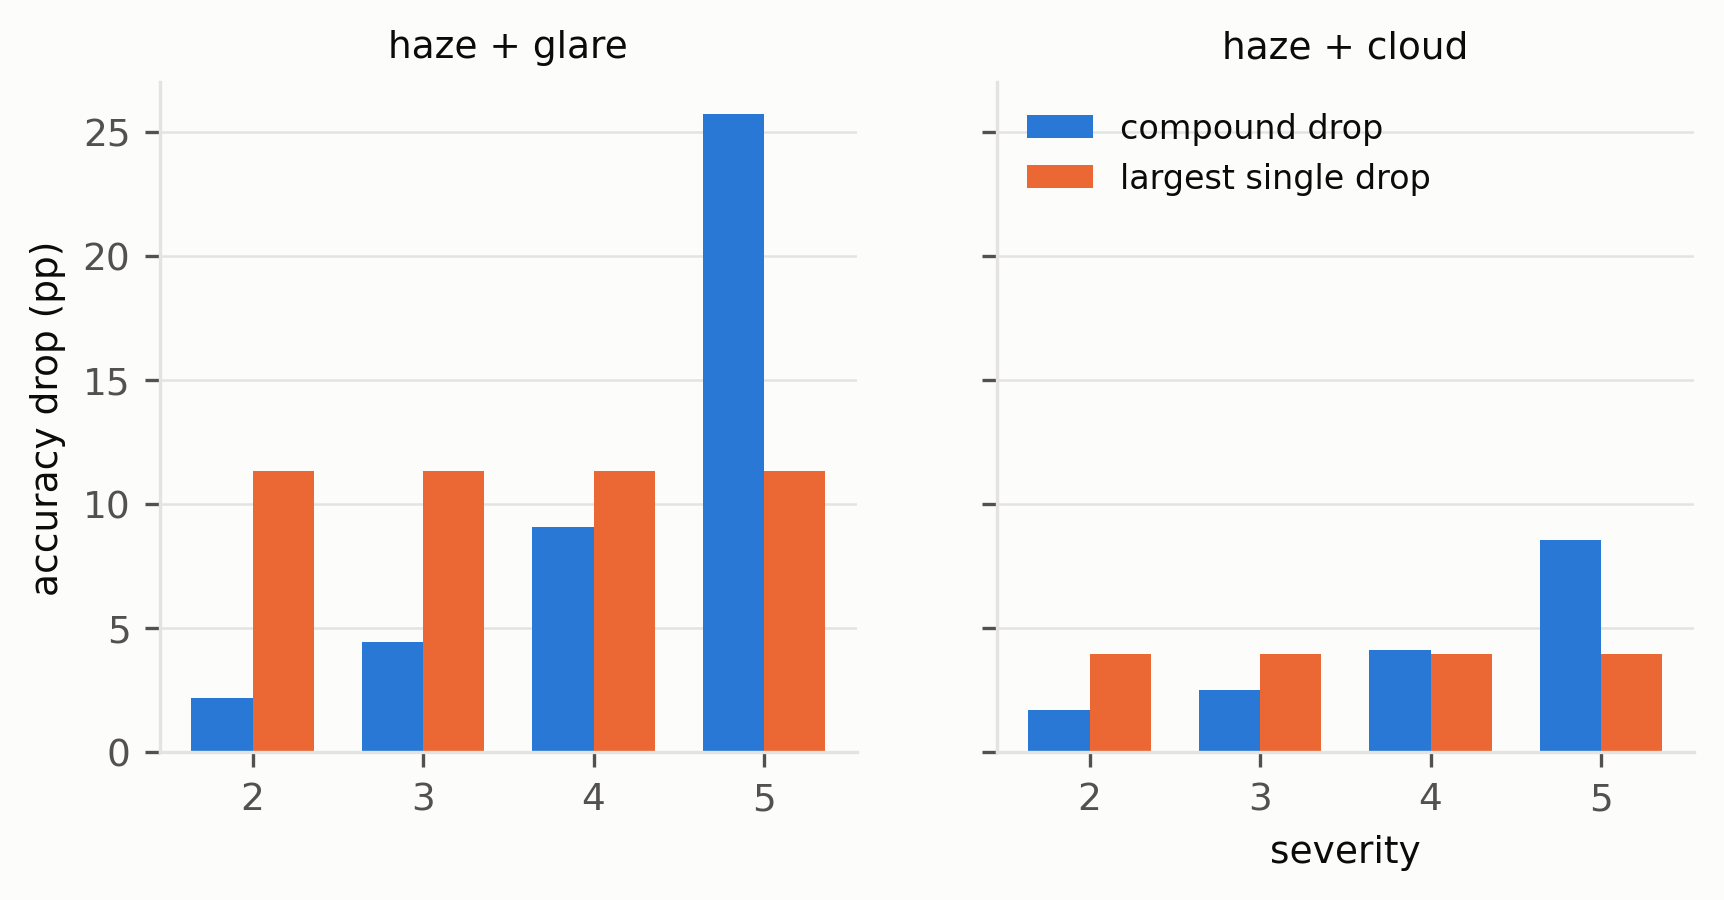
\includegraphics[width=0.78\linewidth]{figures/fig2_compound_vs_single}
\caption{Accuracy drop (pp) of each compound condition against the largest drop produced by any severity of either constituent, baseline arm, mean over 3 folds $\times$ 2 seeds.}
\end{figure}
At severity 5, haze+glare drops accuracy by 25.7 pp and haze+cloud by 8.6 pp, against largest single drops of 11.3 and 4.0 pp. Across four backbone families the same condition (\texttt{matched\_haze+glare\_5}) produces drops between $-$26.1 and $-$43.3 pp, and nine conditions have a mean drop of at least 5 pp with an interval excluding zero in all four: the compound effect is not a property of one architecture.

\subsection{Superadditivity appears at severity 5 only --- a threshold, not a gradient}
We define superadditivity in accuracy space as

E(s) = [acc(clean) $-$ acc(a+b, s)] $-$ {[acc(clean) $-$ acc(a, s)] + [acc(clean) $-$ acc(b, s)]},

so that E(s) is the share of the compound drop not explained by the two marginal drops. The additive baseline sums those marginals, each measured on the same images, model, seed, severity and domain as the compound. Since any such measure could be an artefact of the metric, we report it in accuracy space; the margin-space version appears in Appendix B and agrees in sign.

\noindent\resizebox{\columnwidth}{!}{%
\begin{tabular}{lllll}
\toprule
Severity & haze+glare E & 95\% CI & haze+cloud E & 95\% CI \\
\midrule
2 & 0.00 & [$-$1.45, +1.38] & $-$0.97 & [$-$2.36, +0.41] \\
3 & 0.00 & [$-$2.34, +2.20] & $-$0.49 & [$-$2.20, +1.21] \\
4 & +1.46 & [$-$1.30, +4.24] & +1.21 & [$-$0.98, +3.42] \\
5 & \textbf{+11.33} & \textbf{[+7.22, +15.22]} & +1.62 & [$-$0.97, +4.33] \\
\bottomrule
\end{tabular}}
Only haze+glare at severity 5 survives Benjamini--Hochberg correction over the eight estimates (q < 0.001); all others have q $\geq$ 0.48.

We pre-registered four predictions before running severities 2 and 4. Three are confirmed and one \textbf{failed}; per-run values are in \path{reports/COMPOUND_ANALYSIS.md}:

\begin{itemize}
\item P2 (E at severity 2 covers zero): \textbf{confirmed}.
\item P3 (lower CI bound at severity 5 exceeds 2 pp): \textbf{confirmed} ([+7.22]).
\item P4 (novelty share increases with severity): \textbf{confirmed} (3.8\% $\to$ 6.6\% $\to$ 19.1\% $\to$ 41.5\%).
\item P1 (E increases monotonically with severity in at least five of six runs): \textbf{failed --- 2/6}. The pooled mean is ordered, but the run-to-run noise ($-$3.4 to +4.9 pp at severities 2--4) exceeds the difference between adjacent severities.
\end{itemize}
We report P1's failure rather than redefining the test, because it changes the claim: the data do not support "superadditivity grows with severity" but the sharper \textbf{at severities 2--4 the compound effect is additive, and at severity 5 it is not.} In all six runs E(5) exceeds every E(s $\leq$ 4) of the same run; with no point at severity 4.5, the crossover lies between 4 and 5 and cannot be localised further.

This statement is scoped to one rendering: under an independent, physically-motivated renderer with severity matched on transmission and saturated-pixel fraction, the severity-5 excess is preserved but its onset moves to severity 4. What survives is the excess and its growth; the onset is a property of the renderer (§8.4).

\subsection{Compound failures are new failures}
For each compound condition we ask, per image and per seed: is this image misclassified under the compound, and is it also misclassified under \emph{any} severity of either constituent? The share of such new errors rises with severity from 3.8\% to 6.6\%, 19.1\% and \textbf{41.5\%} for haze+glare and from 1.0\% to 5.5\%, 7.2\% and 22.9\% for haze+cloud (per-condition counts in Appendix E).

Counts are per (fold, seed) evaluation, summed over the six runs; they share images across seeds and are descriptive, not independent. For the severity-3 and severity-5 conditions we additionally compute the overlap with the strongest single condition: 73.4\% and 44.4\% respectively for haze+glare (\path{reports/COMPOUND_ANALYSIS.md}).

Four in ten of the severity-5 haze+glare errors are errors that no single degradation produces on that image --- not even the strongest one, at any severity. \textbf{Scope:} it is bounded by the comparison set actually run --- three families $\times$ five severities $\times$ two domains, the same model and seed --- and says nothing about whether some single degradation outside it could produce them. Nor is it explained by the compound being simply more severe, since no single degradation of comparable severity exists (compound drop 25.7 pp against a largest single drop of 11.3 pp, in all six runs).

This is a behavioural analysis: it does not say \emph{why} the combination produces new errors, and the candidate mechanisms (feature loss at the boundary between two degradation fields, attention displacement by the glare point source under haze, class-boundary motion) are untested.

\subsection{Where the excess comes from: two probes and their limits}
The first probe measures the degradation pipeline, not the model. Over the 23 \texttt{matched} conditions, haze+glare at severity 5 saturates 60.2\% of pixels (any channel $\geq$ 0.99) against 38\% for the most saturated single condition, and is the only condition combining high saturation with low contrast (luminance s.d. 0.094). Fitting the condition-level drop to saturation fraction and contrast gives \textbf{R$^2$ = 0.80} (+30.7 / $-$16.7 pp); an interaction term raises it only to 0.814. Two boundaries apply: it is a \textbf{condition-level} relation, since per-image correlation between saturation and misclassification is only 0.13 and 0.26; and it is incomplete, since haze+cloud at severity 5 saturates nothing, still exceeds the additive prediction and is the largest residual of the fit ($\approx$6 pp).

The second probe asks whether hard highlight clipping --- the mechanism the first points at --- produces the excess. Everything is recomposed as \texttt{corrupt()} does, except that highlights roll off softly above 0.7 instead of clipping at 1.0, with marginal drops re-measured in the same re-rendered world: the haze+glare\_5 excess falls from +9.7 to +6.3 pp (saturation 60.2\% $\to$ 40.7\%). About a third of the excess is hard clipping; the rest survives without it. Single fold and seed, so directional rather than an estimate.

Turning the reading into a model change fails: a fourth input channel marking clipped pixels (zero-initialised mask stem, +1536 parameters), trained on the baseline recipe and scored on the same 43 paired conditions, moves compound accuracy by +0.61 pp (p = 0.43) and +0.97 pp (p = 0.27) on the two seeds, costs single-degradation accuracy ($-$0.47, $-$0.29 pp) and changes sign between seeds on the worst condition ($-$1.9 / +5.8 pp).

Together the three probes support one statement only: saturation and contrast describe the severity-5 drop well \textbf{at the level of conditions} and poorly at the level of images. We do not claim a mechanism for the new errors.

\subsection{The interaction is additive over corruption families}
Everything above concerns three hand-picked degradations. To ask whether the failure of additivity has structure beyond them, we added six synthetic families (defocus, motion, noise, rain, pixelate, impulse) with continuous levels, each calibrated so that alone it costs a matched 10 or 20 pp on the frozen baseline, and measured all fifteen pairs over three folds $\times$ two seeds.

Raw \texttt{E} conflates interaction with error overlap: two degradations that break the same images cannot add up. Against the independent-failure baseline \texttt{delta = e(a+b) $-$ |E\_a $\cup$ E\_b|}, the severity-5 haze+glare excess survives in all six cells (fold0/1/2 $\times$ seed17/29; +7.3 to +13.1 pp, mean +9.9), while haze+cloud falls to $-$0.7 pp; at severities 2--4 both compounds sit 0.4--2.3 pp \emph{below} the union baseline. The headline result is not an artefact of overlap, but haze+cloud should not be called superadditive.

Across the fifteen added pairs, delta ranges from $-$4.4 to +18.3 pp (ConvNeXt-T). A per-family additive model \texttt{delta(a,b) $\approx$ m\_a + m\_b} explains R$^2$ = 0.48--0.90 in all six cells and 0.42--0.75 in all six ResNet-50 cells: which pair fails is largely predicted by which families it contains. The family values do not transfer between backbones (impulse +1.7 pp on ConvNeXt, $-$8.2 pp on ResNet-50), so superadditivity belongs to a (model, corruption) pair, not to a corruption pair alone. No single-corruption geometric predictor recovers the ordering --- mean feature-shift cosine, per-image displacement alignment, retained high-frequency energy and per-class error correlation all fail (|$\rho$| < 0.6 with unstable sign across cells). Predicting which composition will explode requires measuring part of the composition.

A six-cell replication gate fixed before folds 1--2 were run passed four of five criteria on ConvNeXt-T (the failed one, sub-additivity of two low-pass families, held in 4/6 cells); the ResNet-50 study passes all five but was not pre-registered.

\subsection{The same measurement on a standard corruption benchmark}
Everything above rests on one dataset and on families written for this study. Since the decomposition is a measurement claim, we repeat it on CIFAR-10-C \cite{hendrycks2019imagenetc}: fifteen canonical corruptions at five published severities, a ResNet-18 \cite{he2016resnet} trained on clean CIFAR-10 \cite{krizhevsky2009cifar} and evaluated on 601 conditions --- clean, 75 single, 525 pair --- each on the full 10,000-image test set, with per-image correctness stored so every decomposition can be recomputed offline. Nothing here is trained for robustness: the reference model sees clean images only, the setting the compound-corruption literature measures.

Two quantities are computed per condition: \texttt{super = e(a+b) $-$ e(a) $-$ e(b)}, the accuracy-space superadditivity the literature reports, built on additivity of marginal errors; and \texttt{delta = e(a+b) $-$ |E\_a $\cup$ E\_b|}, our union baseline, built on additivity of error \emph{sets}. They differ by exactly the overlap, \texttt{delta $-$ super = |E\_a $\cap$ E\_b|}: the comparison is between two assumptions about what a second corruption does to an error already made.

The archive's generator is unseeded, so infidelity is checked by comparing accuracy on regenerated against published corruptions: 74 of 75 cells agree within the pre-registered 1.0 pp tolerance (worst 1.17 pp, snow at severity 4). Five predictions (C1--C5) were frozen before the grid ran, with the specification that a failure of C1 --- no positive excess at all --- would demote the maritime result to a single-dataset observation.

\textbf{Result.} Over the 525 pair conditions the mean \texttt{delta} is \textbf{+3.63 pp} (median +2.84, 62\% of cells positive, p10--p90 $-$9.5 … +18.8), inside the pre-registered [0, +8] band (C1). The same cells give a mean \texttt{super} of \textbf{$-$7.76 pp}: by the additive baseline the compound is \emph{easier} than its parts, by the union baseline harder, and the gap on identical data is the overlap --- 11.4 pp counted twice. Severity is not monotone (C5): \texttt{delta} climbs through +0.66, +2.93, +4.90, +6.58 and falls to +3.06 at s5. Fog, snow and frost pairs sit 4.2 pp above the median (C4). One prediction \textbf{fails}: \texttt{delta} correlates only $\rho$ = +0.26 with compound damage (C3, threshold 0.3), so the excess is not a law of how damaged the image is. Family signs split --- contrast +10.9, fog +10.5, gaussian noise $-$5.2 --- without following from single-corruption strength.

\textbf{Does covering it transfer, and is it competitive?} Five further arms apply §5's intervention here: pools of 15 and 40 pairs with five pairs held out of both, a singles arm showing every corruption alone at the same rate, and AugMix \cite{hendrycks2020augmix} with its Jensen-Shannon term --- the standard augmentation answer to CIFAR-10-C, at the same 200 epochs and on the same grid. Table 1 gives absolute accuracy, the number a reader compares against published robustness results.

\noindent\resizebox{\columnwidth}{!}{%
\begin{tabular}{lrrrrr}
\toprule
arm & clean & singles & pairs & held-out s3 & held-out delta \\
\midrule
clean reference & 95.47 & 74.77 & 57.29 & 61.14 & +7.86 \\
lattice k=15 & 94.28 & 91.80 & 87.88 & 89.86 & $-$0.17 \\
lattice k=40 & 94.16 & 91.95 & 88.52 & 90.16 & $-$0.42 \\
singles & 94.99 & 92.30 & 86.77 & 90.04 & +0.33 \\
AugMix & 95.36 & 88.95 & 78.72 & 84.84 & +1.97 \\
field bank, 15 families named & 95.05 & 90.76 & 84.66 & --- & --- \\
field bank, 3 families withheld (§4.8) & 94.55 & 90.88 & 85.43 & --- & --- \\
\bottomrule
\end{tabular}}
\emph{Table 1. Percent correct over the 601-condition grid, and the excess on the five held-out pairs at severity 3. All arms at seed 17; second seeds and pair-level bootstrap intervals are in Appendix C.}

Coverage is worth \textbf{30.6 pp} on compound conditions (pair-level bootstrap 95\% CI [+28.5, +32.7]) and 28.7 pp on held-out pairs, for 1.2--1.3 pp of clean accuracy (B3 holds), reproduced at a second seed to within 0.1 pp. It is monotone in pool width but saturates --- k=15 to k=40 buys 0.25 pp (B1 holds) --- so the pool need not be wide, only complete. The pairing contrast fails and stays failed: singles sit at +0.33 pp of excess against the paired arm's $-$0.17, differences of $-$0.49 and $-$0.89 pp, both inside the pre-registered [$-$1, +1] band (B2 fails). Family exposure recovers 7.5--8.3 pp of the 8.0 available; co-occurrence adds under 1 pp, so §5's claim is family coverage, not pair coverage.

\textbf{What this comparison licenses.} AugMix never sees the test corruption families: it reaches 78.72\% on compounds, 9.2 pp below the coverage arms on 104 of 105 pairs (95\% CI [+8.0, +10.4]), its excess is untouched at +4.41 pp, and the coverage arms lead it on singles too (91.8 vs 89.0). The gain is not free augmentation --- it comes from training on the families being evaluated. §4.8 asks how much of it survives when they are not named.

A control separates "trained on augmentations" from "trained on \emph{these} corruptions": \texttt{otheraug} runs the same recipe and epochs on families disjoint from the fifteen evaluated ones. It reaches 69.85\% on compounds --- 12.2 pp above the clean reference, 8.9 below AugMix --- with held-out excess +5.78 pp against +7.86 for the clean reference and +1.97 for AugMix, and all three frozen predictions hold. Augmentation strength is not the variable that moves compound accuracy.

\subsection{Coverage from unlabeled deployment images}
The arms above need the families' names to build a pool; deployment offers images and no list of what will go wrong. \textbf{Field model.} A degradation is written as one composition, \texttt{x\_deg = k * (K ⊙ x\_clean) + N + noise} --- a per-image anisotropic Gaussian convolution \texttt{k}, coarse gain \texttt{K} and additive fields \texttt{N} on an 8$\times$8 grid, and a noise scale. An encoder regresses all of these from a single degraded image on a continuous prior supervised by the generator's own draws, so nothing in training is indexed by family. Run over a pool of unlabeled deployment images it yields a bank of fields; training samples one or two, composes them in field space, and applies the composition to clean images (Fig. 2), with the application count fixed by matching the pool's PSNR --- never by accuracy.

\begin{figure}[t]
\centering
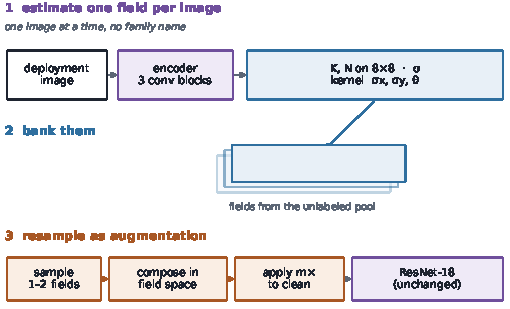
\includegraphics[width=1.0\linewidth]{figures/fig6_ncf_architecture}
\caption{No family name, clean reference or label enters the module: fields are estimated one image at a time, banked from unlabeled deployment images, and resampled --- one or two per sample, composed, applied m times --- as the augmentation of an otherwise unchanged ResNet-18.}
\end{figure}
The bank reaches \textbf{84.66\%} on compounds from a pool that names nothing, and \textbf{85.43\%} when fog, frost and snow are withheld from the pool altogether --- 6.7 pp above AugMix and 2.45 pp below the k=15 lattice; on pairs containing the withheld families it holds 84.96\% against 78.46 for AugMix and 87.64 for the lattice. Clean accuracy is 95.05\% and 94.55\%, the latter clearing its 94.5\% floor by 0.05 pp --- marginal, not comfortable.

The convolution term is what makes this work, confined to the families that need it. Without it the same bank reaches 77.61\% and the five blur and pixelate families sit below AugMix (motion 83.2 vs 92.6); with it they reach 92.5, 93.0, 93.8, 80.3 and 88.5, while noise and photometric families move by under 0.3 pp. The boundary was representational, not family identity.

\section{Coverage: the excess is an operating point training never visits}
The union decomposition of §4.6 says what the excess is not: compound images are not merely harder instances of existing errors. This section asks what removes it, under a deliberately unglamorous hypothesis --- a model can only learn a joint operating point if training shows it one. Under the project's combined recipe, compounds are a quarter of the batches and are drawn from three families (haze, cloud, glare), while the fifteen-pair lattice of §4.6 uses six families that training never mixes. If the excess is an uncovered operating point, teaching the model co-occurrence should remove it --- and teaching it the same families one at a time should not.

\textbf{Design.} Six synthetic families (defocus, motion, noise, rain, pixelate, impulse), each calibrated so that the level parameter swept until a single family alone costs 20 pp on validation. Three of the fifteen pairs (\texttt{noise+pixelate}, \texttt{defocus+rain}, \texttt{motion+impulse}) are held out of every training pool, so nothing below is evaluated on a pair the model could have memorised; nested balanced pools \texttt{c3}, \texttt{c6} and \texttt{c12} contain 3, 6 and 12 distinct pairs over the remaining twelve. Every arm --- including the re-measured baseline --- gives each sample a clean view with probability 0.5 and a compound otherwise, so \emph{compound exposure is held constant} and only the diversity of the compound distribution varies. Three folds $\times$ two seeds, 40 epochs, ConvNeXt-T, identical to §3.

\textbf{Result.} On the three held-out pairs the baseline excess is +8.2 pp (clean accuracy 84.95\%). A pool of three pairs takes it to \textbf{$-$1.8 pp} (86.25), six pairs to +2.0 (86.08), twelve pairs to +1.4 (86.41). The excess is removable: a handful of the right operating points turns an 8.2-pp excess into one of the opposite sign at no clean-accuracy cost. And our pre-registered dose-response prediction (P2: monotone improvement with pool size) \textbf{failed}: three pairs is as good as, or better than, twelve, by +3.5 pp (sd 2.2, 6 cells). What matters is not how many pairs the pool holds but whether each family appears in at least one --- every pool here contains all six, and extra pairs add nothing. All eight arms, with the pair-level numbers, are in Appendix F.

\begin{figure}[t]
\centering
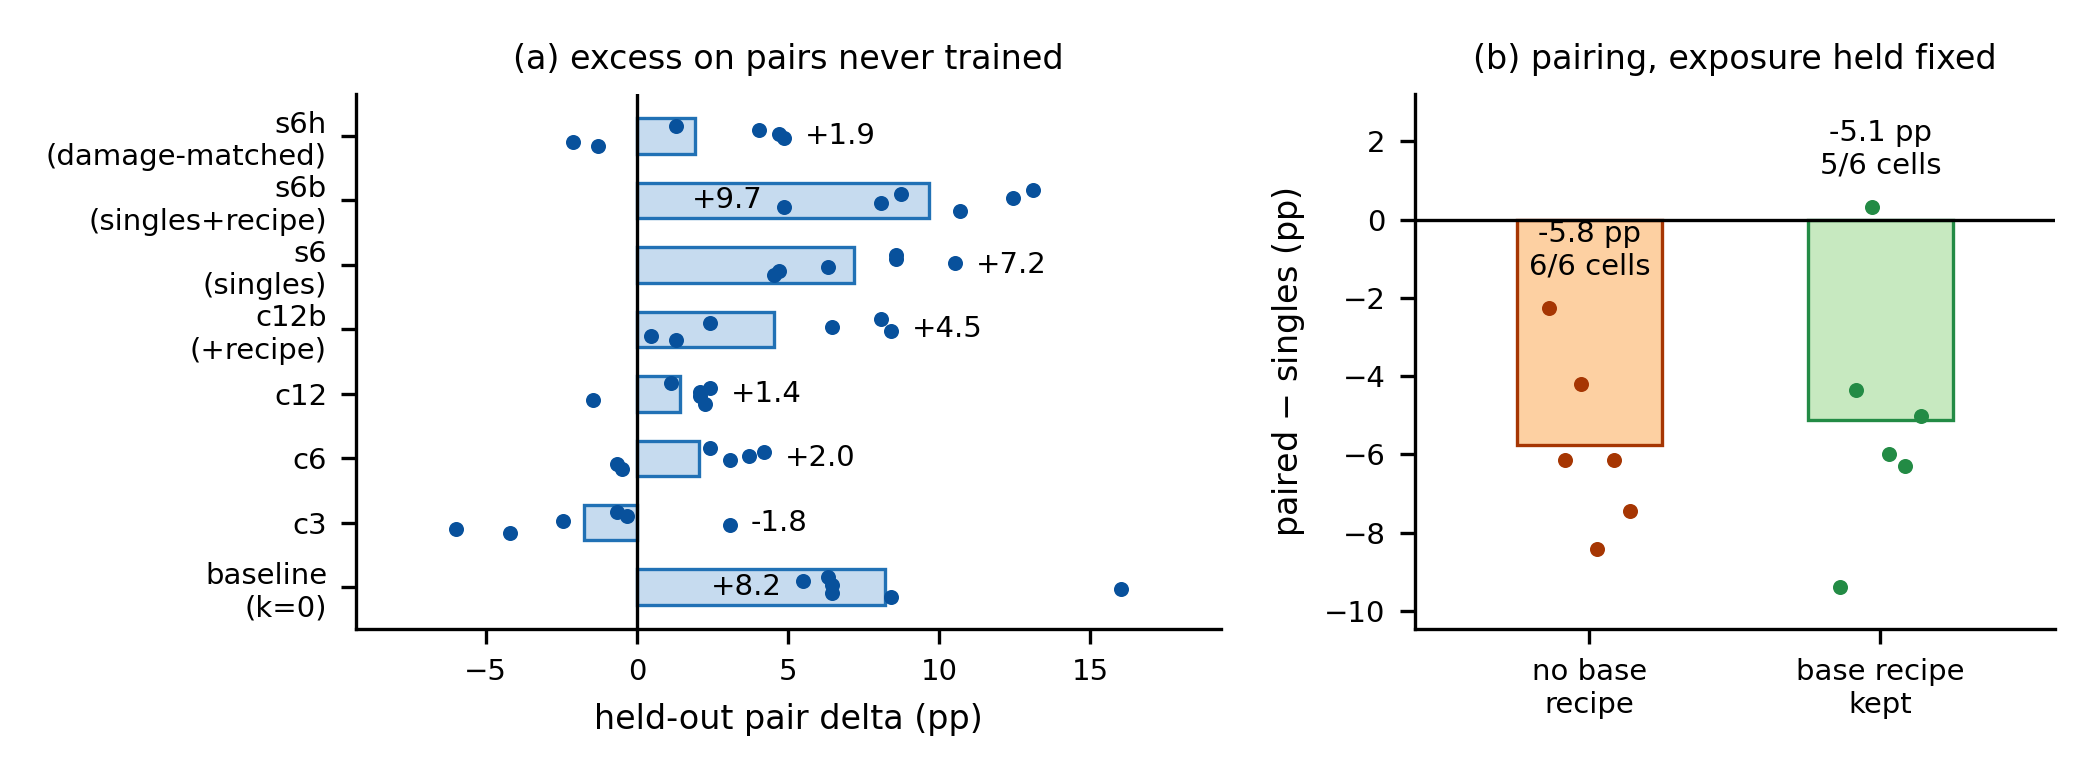
\includegraphics[width=0.70\linewidth]{figures/fig5_coverage}
\caption{(a) Excess on the three held-out pairs for each arm, one dot per (fold, seed) cell; (b) the paired-minus-singles contrast, in which compound exposure is identical by construction, for the two recipe settings. Negative is better: it means the pair arm has less excess than the same families applied one at a time.}
\end{figure}
\textbf{What the gain is not.} Family exposure is the obvious alternative explanation, so \texttt{s6} applies the same six families at the same 50/50 rate, one per draw instead of two: it lands at \textbf{+7.2 pp} (clean 86.73), almost exactly the baseline. Against \texttt{c12} the paired-minus-singles difference is \textbf{$-$5.8 pp (range $-$8.4 to $-$2.3), negative in 6 of 6 cells}; on the twelve pool pairs $-$5.1 pp; clean accuracy differs by $-$0.3 pp. The result also holds when the project's own combined recipe is kept in the mixture rather than replaced: \texttt{c12b} reaches +4.5 against \texttt{s6b}'s +9.7, a paired-minus-singles difference of \textbf{$-$5.1 pp} (5/6 cells negative, pool pairs $-$6.0 pp, 6/6).

\textbf{Damage per image is a real confound, and it is part of the effect.} A compound image carries roughly twice the damage of a single-family image. We removed this in a third control: \texttt{s6h} applies one family per draw at a level calibrated so that a \emph{single} corruption costs 40 pp, the same damage per image a pair carries. It reaches \textbf{+1.9 pp} (clean 86.08). Our pre-registered prediction (P12: $\geq$ +3.0 pp, i.e. that damage-matching would not reproduce the gain) is \textbf{falsified}: matching the damage recovers 5.3 of the 8.9 pp that separates \texttt{s6} from \texttt{c3}. What survives is smaller but consistent --- at equal damage per image, pairs still beat singles by \textbf{$-$3.7 pp (range $-$7.1 to $-$1.8), 6 of 6 cells}, on pairs seen in no training pool. The honest decomposition of the 8.9-pp gain is therefore roughly 60\% damage per image and 40\% co-occurrence, and only the co-occurrence part survives matching.

\textbf{Where it stops.} Coverage removes the excess only for pairs drawn from families the pools cover. The paper's haze+glare condition is in no lattice and its families are absent from the lattice recipe: with the base recipe retained (\texttt{c12b} vs \texttt{s6b}), its severity-5 accuracy is 56.1\% against 57.4\% and its excess 11.0 pp against 12.0 pp, no improvement, as the pre-registered negative prediction (P10) expected. Coverage transfers to unseen \emph{pairs} over covered \emph{families}, not to unseen \emph{families} --- a boundary of the mechanism, not a defect of the experiment: covering the compositions at the families you expect to meet is the operative recipe.

\section{Interventions: a pre-registered negative result}
Seven interventions across three loci plus one initialization control, each trained at 40 epochs, three folds, two seeds, with identical data, preprocessing, corruption instances and evaluation. Screening criteria were fixed in advance: mean gain $\geq$ +1.5 pp on the combined conditions, two of three folds positive, no clean-accuracy loss beyond 1 pp, and a paired bootstrap interval excluding zero. All eight fail it: the best candidate is I1 at +0.94 pp [$-$0.09, +1.98], and seven of the eight are negative, down to T3 at $-$8.76 pp. The full table is Appendix D.

Two caveats we insist on. First, R1's interval covers zero: the correct statement is "no detectable gain at +4\% parameters and +8.5\% latency", not "significant harm". Second, T4 compares two specific weight sets, not "pretraining quality" as a factor.

\textbf{The budget artefact.} T1 showed +1.66 pp [0.63, 2.68] when screened at 24 epochs and $-$0.18 pp [$-$1.13, 0.76] at 40 epochs. Both arms improved with the longer budget (84.5 $\to$ 85.7 and 84.0 $\to$ 85.1 macro-F1), so the candidate's apparent advantage was the difference between two convergence trajectories. Any pipeline comparing candidates at a truncated budget inherits this risk; full-budget confirmation caught it.

\textbf{Error-flow analysis.} Across 6 (fold, seed) pairs $\times$ 8 conditions $\times$ 206 images, every candidate fixes some baseline errors and breaks more: R1 620 fixed / 728 broken, I2 639/904, T2 608/1103, T3 547/1415 (descriptive; the counts are not independent). Clean accuracy does not rank candidates either: the curriculum arm had the best clean accuracy (85.1\%) and the worst compound accuracy (67.3\%), and the ImageNet-22K initialization gained +0.73 pp clean while losing $-$0.71 pp compound --- an argument against selecting models by clean validation accuracy when deployment is under weather.

\section{Real imagery: observational only}
On 157 FGSC-23 validation images annotated for real degradation (93 with at least one), the accuracy difference between degraded and clean groups is $-$2.3 pp, seed interval [$-$7.8, +4.3]; on 184 two-class FGSRCS development crops it is +1.8 pp. Neither can support a claim that real degradation hurts accuracy here --- the heavy-degradation stratum holds at most two images --- so we report them only to bound the claim: the findings concern the synthetic protocol, not their transfer to real weather.

\section{Discussion and limitations}
\subsection{What this work supports}
\begin{itemize}
\item Compound degradations are not additive at the highest severity: the joint drop exceeds the sum of marginals by 11.3 pp and 41.5\% of severe-compound errors come from no single degradation --- not mere difficulty.
\item The excess is not intrinsic. A pool over the same six families turns +8.2 pp of held-out excess into $-$1.8 pp at no clean cost, where the same families applied one at a time leave +7.2 pp; about 40\% of that gain survives damage matching, and only that part transfers to unseen pairs. On CIFAR-10-C, single families recover the same 8.3 pp (§4.7), and a pool built from unlabeled images without family names recovers 6.7 pp above AugMix (§4.8).
\item Seven mechanism-diverse single-point interventions and one initialization control do not beat a strong combined-augmentation baseline; the negative result is pre-registered and reproducible.
\end{itemize}
\subsection{What it does not support}
\begin{itemize}
\item \textbf{No performance ceiling.} Frequency-domain methods, deeper backbones, larger data and multi-factor interventions were not tested; the best arm here is not a state-of-the-art claim.
\item \textbf{No mechanism.} The novelty analysis is behavioural. The saturation/contrast fit of §4.5 is a condition-level association (R$^2$ = 0.80) with weak per-image correlation (r = 0.13, 0.26), and every mechanism test is negative or partial: removing hard clipping removes a third of the excess, a clipped-pixel mask gives no gain, and a drift signal that predicts failure (AUC 0.78--0.82) fails as a training weight. The mechanism behind new errors is unknown.
\item \textbf{No established threshold.} "Threshold" is an inference from four severity levels: the crossover is bounded only to (4, 5), and our pre-registered monotonicity prediction failed (P1, 2 of 6 runs). A physically-motivated re-rendering (§8.4) moves the onset to severity 4 while preserving the severity-5 excess, so the claim is descriptive --- an excess that grows with severity --- not a law of the axis.
\item \textbf{No generalization to real weather.} §7 is observational with insufficient heavy-degradation samples.
\item \textbf{No transfer across families.} Coverage removes the excess on pairs drawn from families the pools contain, not on haze+glare, whose families are absent from every lattice pool (§5, P10): a deployment recipe must cover the degradations it expects to meet.
\end{itemize}
\subsection{Data disclosure}
The 236 images in FGSC-23's \texttt{test} split were used by three diagnostic analyses on 2026-10-29 (part occlusion, recovery, restoration). They were not used in training or in any number here, but they are \textbf{no longer an unseen test set} and this paper does not call them one.

\subsection{Threats to validity}
Single dataset; 618 training images; two seeds; five severity levels with nothing between 4 and 5.

\textbf{Two renderers, not one.} Re-rendering haze with Koschmieder depth transmission and glare with a specular lobe plus blooming, severity matched on mean transmission and saturated-pixel fraction, gives E(5) = +14.6 / +21.8 pp on the frozen baseline and +10.2 / +16.0 pp after retraining; only \texttt{haze+glare} is re-rendered. The excess belongs to the interaction, not to one clipping model, though the \emph{onset} moves to severity 4 and saturation matching pins the saturated fraction by construction, so the experiment shows spatial structure matters at fixed saturation, not that saturation is the cause. Remaining caveats: the cloud implementation, one backbone family and one fold in the physical test, and a bootstrap over images only, not the condition grid.

\section{Conclusion}
Compound weather degradations do what singles do not: at the highest severity the joint effect exceeds the additive prediction by 11.3 pp and 41.5\% of the errors come from no single degradation; at moderate severities they are additive. On CIFAR-10-C the additive convention reverses the union baseline's sign ($-$7.8 against +3.6 pp); the gap is error overlap counted twice. Coverage removes the excess given the families --- \textbf{+30.6 pp} of compound accuracy for 1.2 pp of clean accuracy, against +21.4 pp for AugMix --- and a field bank estimated from unlabeled deployment images recovers 6.7 pp of it without names. Predictions and negative results are released together.

